\subsection{Kinematics and dynamics for quantum spin chains with defects}\label{Kin_Dyn}

Our goal in this introductory subsection is to present a framework to make physical and microscopic sense of a dynamical theory of defects for quantum (spin) systems. We restrict our attention to defects modeled by absent/missing quantum spins. (Extending this idea to more general defects modeled by different Hilbert spaces then becomes a straightforward task.)

Firstly, we focus on the problem of modeling an \emph{indefinite} number of distinguishable spins. Building on this we can propose a kinematical space to model arbitrary numbers of quantum spins at various locations. This allows us to then consider the case of missing-spin defects for topologically ordered systems.

When we want to describe a quantum system with an \emph{indefinite} number of \emph{indistinguishable} particles we should use \emph{Fock space}. We will use the arguably conceptually simpler construction of \emph{distinguishable Fock space} (see \cite{OsborneVideoLectureAQT} for a course where this is explained), appropriate for describing a collection of an indefinite number of distinguishable particles. Subsequently, one can obtain Bose-/Fermi-Fock space by imposing an equivalence relation under particle exchange. Distinguishable Fock space is given by
\begin{equation}
\mathfrak{F}(\mathbb{C}^d) \cong \bigoplus_{N=0}^\infty \mathcal{H}_N\cong \bigoplus_{N=0}^\infty (\underbrace{\mathbb{C}^d\otimes \mathbb{C}^d\otimes \cdots \otimes \mathbb{C}^d}_{\text{$N$ factors}}),
\end{equation}
where $\mathcal{H}_N$ is the Hilbert space for $N$ distinguishable particles. By convention and assumption the space describing zero particles, the \emph{vacuum}, is assigned the Hilbert space $(\mathbb{C}^d)^{\otimes 0} \cong \mathbb{C}$.

It is now easy to incorporate additional constraints on the numbers of particles, e.g., to describe a system comprised of \emph{either} zero distinguishable quantum spins \emph{or} one distinguishable quantum spin we would use
\begin{equation}
\mathfrak{F}_{\le 1} (\mathbb{C}^d) \cong \mathbb{C}\oplus \mathbb{C}^d.
\end{equation}
We could call this the Hilbert space of a ``maybe'' quantum spin.

Let's now consider the central situation for this work. How should we describe a quantum lattice of $n$ sites, where either a single quantum spin is present at a site, or not? (We call the case where a spin is absent a \emph{defect}.) According to the discussion above we should simply tensor up $N$ ``maybe'' quantum spins:
\begin{equation}
\mathfrak{F}_{\le n}(\mathbb{C}^d) \equiv \bigotimes_{N=0}^n \mathfrak{F}_{\le 1}(\mathbb{C}^d) \cong (\mathbb{C}\oplus \mathbb{C}^d)^{\otimes N}.
\end{equation}
Expanding out the tensor factors leads to the equivalent definition
\begin{equation}
\mathfrak{F}_{\le n}(\mathbb{C}^d) \equiv \bigoplus_{j=0}^N \mathbb{C}^{\binom{N}{j}}\otimes \mathcal{H}_j.
\end{equation}
The Hilbert space $\mathfrak{F}_{\le n}(\mathbb{C}^d)$ supplies us with just the kinematical data to describe a system of distinguishable particles. To incorporate additional dynamical information we must specify additional \emph{dynamical} data.

In the context of topologically ordered models such as Kitaev's toric code \cite{Kit03} we typically introduce dynamical information indirectly by describing the system via the ground eigenspace $\mathcal{V}\subset \mathcal{H}$ of a specific Hamiltonian $H$. In the case of the toric code for $N\times N$ quantum spins arranged on the torus, the ground eigenspace $\mathcal{V}_{\mathbb{T}}$ of the toric code Hamiltonian is four dimensional. Let us now assume we have a lattice with a missing-qubit defect at some edge $e$ \cite{BLKW17}, see Fig. \ref{fig:1defect}. One can define a toric-code Hamiltonian for this new punctured torus; restricting to its ground eigenspace yields a \emph{four-dimensional subspace} $\mathcal{V}_{\mathbb{T}\setminus e}$. There is no obstruction to describing the ground eigenspace for two, three, etc.\ missing-qubit defects. What results is a rather intricate combinatorial problem, as, depending on where the defects are located relative to each other, one gets higher or lower dimensional ground eigenspace. To see an example of the intricacies that easily result, consider the case of two missing edges: these can either be adjacent to each other or distant. In the latter case, depicted in Fig. \ref{fig:2distdefects}, the ground space for this system is $(\mathbb{C}^2)^{\otimes 3}$ while in the case of adjacent defects we have a single larger puncture (with smooth boundary), see Fig. \ref{fig:2adjdefects}, and the ground eigenspace is only $(\mathbb{C}^2)^{\otimes 2}$.

\begin{figure}
	\centering
	\begin{subfigure}[t]{0.3\linewidth}
		\centering
		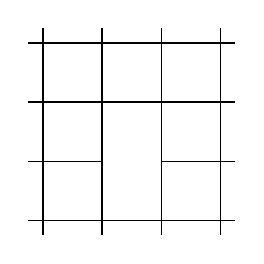
\begin{tikzpicture}[scale=0.75,baseline=(current bounding box.center)]
		%horizontal lines
		\draw (-0.25,0) -- (3.25,0);
		\draw (-0.25,-1) -- (3.25,-1);
		\draw (-0.25,-2) -- (1,-2);
		\draw (2,-2) -- (3.25,-2);
		\draw (-0.25,-3) -- (3.25,-3);
		%vertical lines
		\draw (0,-3.25) -- (0,0.25);
		\draw (1,-3.25) -- (1,0.25);
		\draw (2,-3.25) -- (2,0.25);
		\draw (3,-3.25) -- (3,0.25);
		\end{tikzpicture}
		\caption{One missing qubit defect on a toric code lattice.}\label{fig:1defect}
	\end{subfigure}\vspace{20pt}
	
	\begin{subfigure}[t]{0.3\linewidth}
		\centering
		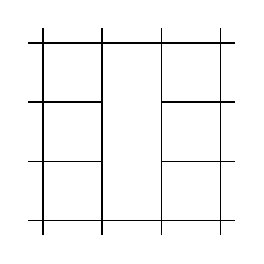
\begin{tikzpicture}[scale=0.75,baseline=(current bounding box.center)]
		%horizontal lines
		\draw (-0.25,0) -- (3.25,0);
		\draw (-0.25,-1) -- (1,-1);
		\draw (2,-1) -- (3.25,-1);
		\draw (-0.25,-2) -- (1,-2);
		\draw (2,-2) -- (3.25,-2);
		\draw (-0.25,-3) -- (3.25,-3);
		%vertical lines
		\draw (0,-3.25) -- (0,0.25);
		\draw (1,-3.25) -- (1,0.25);
		\draw (2,-3.25) -- (2,0.25);
		\draw (3,-3.25) -- (3,0.25);
		\end{tikzpicture}
		\caption{Two adjacent missing qubit defects on a toric code lattice.}\label{fig:2adjdefects}
	\end{subfigure}\vspace{20pt}
	
	\begin{subfigure}[t]{0.3\linewidth}
		\centering
		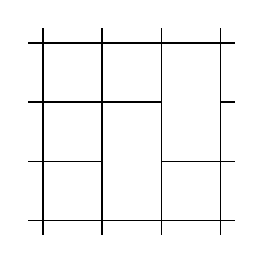
\begin{tikzpicture}[scale=0.75,baseline=(current bounding box.center)]
		%horizontal lines
		\draw (-0.25,0) -- (3.25,0);
		\draw (-0.25,-1) -- (2,-1);
		\draw (3,-1) -- (3.25,-1);
		\draw (-0.25,-2) -- (1,-2);
		\draw (2,-2) -- (3.25,-2);
		\draw (-0.25,-3) -- (3.25,-3);
		%vertical lines
		\draw (0,-3.25) -- (0,0.25);
		\draw (1,-3.25) -- (1,0.25);
		\draw (2,-3.25) -- (2,0.25);
		\draw (3,-3.25) -- (3,0.25);
		\end{tikzpicture}
		\caption{Two distant missing qubit defects on a toric code lattice.}\label{fig:2distdefects}
	\end{subfigure}
	\caption{Depiction of different situations where missing qubit defects are inserted on a toric code lattice. In the case of more than one missing link the ground space for the system depends on whether the defects are adjacent to each other.}
\end{figure}

Writing out the whole ground eigenspace is a highly intricately combinatorial problem, which is why we exploit concepts from category theory to model defects in the system. Of course, the above description is not only restricted to the toric code case. In Sec.~\ref{Ising}, we show how this construction works for a one-dimensional spin system and we also show how ideas and techniques from category theory can be used to model dynamical defects in such a one-dimensional spin system. But for now, let us introduce the basic category theoretical toolbox needed for studying dynamical defects in those spin chains.